%%%%%%%%%%%%%%%%%%%%%%%%%%%%%%%%%%%%%%%%%%%%%%%%%%%%%%%%%%%%%%%%%%%%%
% LaTeX Template: Softwaretechnik SS 2017
%
% Date: April 2017
%
%%%%%%%%%%%%%%%%%%%%%%%%%%%%%%%%%%%%%%%%%%%%%%%%%%%%%%%%%%%%%%%%%%%%%%

\documentclass[12pt]{article}
\usepackage[a4paper]{geometry}
\usepackage{framed}
\usepackage[myheadings]{fullpage}
\usepackage{fancyhdr}
\usepackage{lastpage}
\usepackage{graphicx, wrapfig, subcaption, setspace, booktabs}
% \usepackage{movie15}
\usepackage[T1]{fontenc}
\usepackage[font=small, labelfont=bf]{caption}
\usepackage[protrusion=true, expansion=true]{microtype}
\usepackage[german]{babel}
\usepackage{sectsty}
\usepackage{url, lipsum}
\usepackage[parfill]{parskip}
\usepackage{csquotes}
\usepackage[hidelinks]{hyperref}
\usepackage[acronym]{glossaries}


\makeglossaries
\glstoctrue



%-------------------------------------------------------------------------------
% Commands
%-------------------------------------------------------------------------------
\newcommand{\HRule}[1]{\rule{\linewidth}{#1}}
\input{../env}
%-------------------------------------------------------------------------------
% HEADER & FOOTER
%-------------------------------------------------------------------------------
\pagestyle{fancy}
\fancyhf{}
\setlength\headheight{15pt}
\fancyhead[L]{\newCommandName}
\fancyhead[R]{\newCommandUniversity}
\fancyfoot[R]{Seite \thepage\ von \pageref{LastPage}}

%-------------------------------------------------------------------------------
% TITLE PAGE
%-------------------------------------------------------------------------------
\begin{document}
\hypersetup{
    colorlinks,
    citecolor=black,
    filecolor=black,
    linkcolor=black,
    urlcolor=black
}


\title{ \normalsize
		\HRule{0.5pt} \\
		\LARGE \textbf{\uppercase{\newCommandDiscipline}} \\
    \smallbreak
		\small\textbf{{\newCommandTerm}}\\
		\HRule{2pt} \\ [0.5cm]
		\normalsize \today \vspace*{10\baselineskip}}

\date{}

\author{
		\newCommandName \\
		\newCommandMatriculationNumber \\
		\newCommandUniversity \\
		\newCommandFaculty
}

% \pagenumbering{gobble}

\maketitle
\thispagestyle{empty}

\newpage


\tableofcontents
\newpage



%-------------------------------------------------------------------------------
% Section title formatting
\sectionfont{\scshape}
%-------------------------------------------------------------------------------

%-------------------------------------------------------------------------------
% BODY
%-------------------------------------------------------------------------------

\section{SWT - Einf"uhrung in die Softwaretechnik}

%-------------------------------------------------------------------------------
% #1
%-------------------------------------------------------------------------------

\newglossaryentry{st}{type=\acronymtype, name={ST}, description={Softwaretechnik}}
\newglossaryentry{cmm}{name=CMM, description={Capability Maturity Model}}
\newglossaryentry{pmmm}{name=PMMM, description={Project Management Maturity Model}}

\subsection{"Ubung SWT-01}
\subsubsection*{Aufgabe:}

\begin{framed}
\textbf{Softwaretechnik allgemein}
\smallbreak
Was ist Softwaretechnik? Was wird da gelehrt? Worum geht es?
\\
Was antworten Sie?
\bigbreak
\small Bearbeitungszeit: 10 Minuten
\end{framed}
\bigbreak
\bigbreak
\subsubsection*{L"osung:}

\textbf{Der IEEE-Standard 610-1990 definiert Softwaretechnik als:}


\begin{center}
% \enquote{(1) The application of a \textbf{systematic}, \textbf{disciplined}, \textbf{quantifiable} approach to the development, operation, and maintenance of software; that is, the application of engineering to software. (2) The study of approaches as in (1)}
\enquote{The application of a  systematic\footnote{\label{foot:1}systematic - having, showing, or involving a system, method, or plan}, disciplined\footnote{\label{foot:2}disciplined - having or exhibiting discipline; rigorous}, quantifiable\footnote{\label{foot:3}quantifiable - to determine, indicate, or express the quantity of} approach to the development, operation, and maintenance of software; that is, the application of engineering to software.}
\end{center}

% ``The application on a systematic, disciplined, quantifiable approach to the development, operation and maintenance of software; that is the application of engineering of software''
%
% \begin{itemize}
% \item http://dictionary.reference.com/browse/systematic: having, showing, or involving a system, method, or plan
% \item http://dictionary.reference.com/browse/disciplined: having or exhibiting discipline; rigorous
% \item http://dictionary.reference.com/browse/quantifiable: to determine, indicate, or express the quantity of.
% \end{itemize}
%
% \bigbreak
% \bigbreak
%
% \textbf{Das SEI selbst definiert SE ebenfalls in zwei Schritten als:}
%
% ``Engineering is the systematic application of scientific knowledge in creating and building cost-effective solutions to practical problems in the service of mankind.''
% \\
% ``Software engineering is that form of engineering that applies the principles of computer science and mathematics to achieving cost-effective solutions to software problems.''
% \bigbreak
% \bigbreak
\bigbreak
\bigbreak

Aus dieser Definition k"onnen folgende Merkmale der \gls{st} benannt werden:
\bigbreak
\begin{itemize}
\item ST umfasst Methoden, Techniken und Instrumente zur Erstellung von auf Maschinen lauff"ahigen Programmen (Software).
\item Ziel von ST ist die Vermeidung von Fehlern, Reduktion von Aufw"anden und Erh"ohung des Kundennutzens von Software.
\item ST beinhaltet das Management von Entwicklungsprojekten f"ur Software.
\item ST umfasst die Inbetriebnahme, den Betrieb und die Wartung von Software.
\item Hierzu beschreibt SE bew"ahrte Vorgehensweisen in Modellen (Vorgehensmodelle) und definiert Qualit"atsstufen f"ur den Software-Entwicklungsprozess (\gls{cmm}, \gls{pmmm}).
\end{itemize}









%-------------------------------------------------------------------------------
% #2
%-------------------------------------------------------------------------------
\newpage
\subsection{"Ubung SWT-02}
\subsubsection*{Aufgabe:}

\begin{framed}
\textbf{Softwarelebenszyklus}
\smallbreak
Sie werden in einem Bewerbungsgespr"ach gebeten, die wesentlichen Teile des Softwarelebenszyklus an dem Whiteboard zu skizzieren und zu erl"autern.
\\ K"onnen Sie das?
\bigbreak
\small Bearbeitungszeit: 15 Minuten
\end{framed}
\bigbreak
\bigbreak
\subsubsection*{L"osung:}
Lorem ipsum dolor sit amet, consectetur adipisicing elit, sed do eiusmod tempor incididunt ut labore et dolore magna aliqua. Ut enim ad minim veniam, quis nostrud exercitation ullamco laboris nisi ut aliquip ex ea commodo consequat. Duis aute irure dolor in reprehenderit in voluptate velit esse cillum dolore eu fugiat nulla pariatur. Excepteur sint occaecat cupidatat non proident, sunt in culpa qui officia deserunt mollit anim id est laborum.

%-------------------------------------------------------------------------------
% #3
%-------------------------------------------------------------------------------
\newpage
\subsection{"Ubung SWT-03}
\subsubsection*{Aufgabe:}

\begin{framed}
\textbf{Prinzipien}
\smallbreak
Geben Sie bitte zu jedem Prinzip der Softwaretechnik (Abstraktion, Strukturierung, Hierarchisierung, Modularisierung, Standardisierung) ein Beispiel an. Wo ist Ihnen das schon begegnet und wo k"onnte das in der Softwaretechnik angewendet oder wirksam werden?
\bigbreak
\small Bearbeitungszeit: 10 Minuten
\end{framed}
\bigbreak
\bigbreak
\subsubsection*{L"osung:}
Lorem ipsum dolor sit amet, consectetur adipisicing elit, sed do eiusmod tempor incididunt ut labore et dolore magna aliqua. Ut enim ad minim veniam, quis nostrud exercitation ullamco laboris nisi ut aliquip ex ea commodo consequat. Duis aute irure dolor in reprehenderit in voluptate velit esse cillum dolore eu fugiat nulla pariatur. Excepteur sint occaecat cupidatat non proident, sunt in culpa qui officia deserunt mollit anim id est laborum.

%-------------------------------------------------------------------------------
% #4
%-------------------------------------------------------------------------------
\newpage
\subsection{"Ubung SWT-04}
\subsubsection*{Aufgabe:}

\begin{framed}
\textbf{Recherche}
\smallbreak
Recherchieren Sie bitte im Internet "uber Softwaretechnik oder Softwareengineering. Welche Bereiche interessieren Sie ganz besonders?
\bigbreak
\small Bearbeitungszeit: 30 Minuten
\end{framed}
\bigbreak
\bigbreak
\subsubsection*{L"osung:}
Lorem ipsum dolor sit amet, consectetur adipisicing elit, sed do eiusmod tempor incididunt ut labore et dolore magna aliqua. Ut enim ad minim veniam, quis nostrud exercitation ullamco laboris nisi ut aliquip ex ea commodo consequat. Duis aute irure dolor in reprehenderit in voluptate velit esse cillum dolore eu fugiat nulla pariatur. Excepteur sint occaecat cupidatat non proident, sunt in culpa qui officia deserunt mollit anim id est laborum.

%-------------------------------------------------------------------------------
% #5
%-------------------------------------------------------------------------------
\newpage
\subsection{"Ubung SWT-05}
\subsubsection*{Aufgabe:}

\begin{framed}
\textbf{Wissensfragen zur Lerneinheit}
\smallbreak
Versuchen Sie die Fragen schriftlich zu beantworten ohne noch einmal in der Lerneinheit nachzuschlagen.
\begin{enumerate}
\item An welche Best Practices erinnern Sie sich oder welche haben Sie verinnerlicht?
\item Warum ist es sinnvoll Softwarefehler fr"uh zu erkennen?
\item Was geht in Softwareprojekten typischerweise schief?
\item Kennen Sie (Standardisierungs-)Organisationen, die sich mit Software besch"aftigen?
\end{enumerate}
\bigbreak
\small Bearbeitungszeit: 15 Minuten
\end{framed}
\bigbreak
\bigbreak
\subsubsection*{L"osung:}
Lorem ipsum dolor sit amet, consectetur adipisicing elit, sed do eiusmod tempor incididunt ut labore et dolore magna aliqua. Ut enim ad minim veniam, quis nostrud exercitation ullamco laboris nisi ut aliquip ex ea commodo consequat. Duis aute irure dolor in reprehenderit in voluptate velit esse cillum dolore eu fugiat nulla pariatur. Excepteur sint occaecat cupidatat non proident, sunt in culpa qui officia deserunt mollit anim id est laborum.

%-------------------------------------------------------------------------------
% #6
%-------------------------------------------------------------------------------
\newpage
\subsection{"Ubung SWT-06}
\subsubsection*{Aufgabe:}

\begin{framed}
\textbf{Fehlerquellen}
\smallbreak
H"aufige Fehlerquellen in Softwareprojekten sind:
\bigbreak
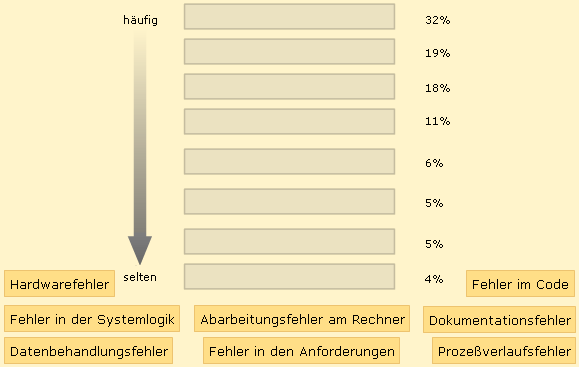
\includegraphics[width=1.0\textwidth]{./images/ueb01-06.png}
\end{framed}
\bigbreak
\bigbreak
\subsubsection*{L"osung:}
Lorem ipsum dolor sit amet, consectetur adipisicing elit, sed do eiusmod tempor incididunt ut labore et dolore magna aliqua. Ut enim ad minim veniam, quis nostrud exercitation ullamco laboris nisi ut aliquip ex ea commodo consequat. Duis aute irure dolor in reprehenderit in voluptate velit esse cillum dolore eu fugiat nulla pariatur. Excepteur sint occaecat cupidatat non proident, sunt in culpa qui officia deserunt mollit anim id est laborum.

%-------------------------------------------------------------------------------
% #7
%-------------------------------------------------------------------------------
\newpage
\subsection{"Ubung SWT-07}
\subsubsection*{Aufgabe:}

\begin{framed}
\textbf{Phaseneinteilung}
\smallbreak
Ordnen Sie die Phasen und Ergebnisse des Softwarelebenszyklus in der richtigen Reihenfolge an.
\bigbreak
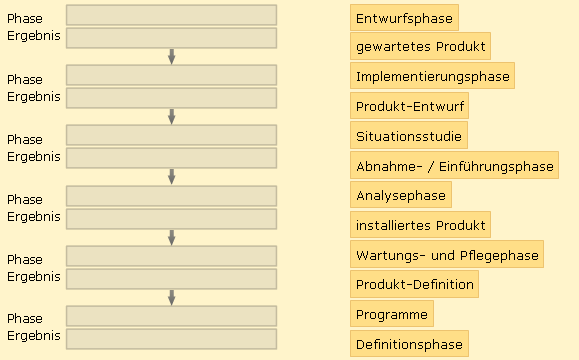
\includegraphics[width=1.0\textwidth]{./images/ueb01-07.png}
\end{framed}
\bigbreak
\bigbreak
\subsubsection*{L"osung:}
Lorem ipsum dolor sit amet, consectetur adipisicing elit, sed do eiusmod tempor incididunt ut labore et dolore magna aliqua. Ut enim ad minim veniam, quis nostrud exercitation ullamco laboris nisi ut aliquip ex ea commodo consequat. Duis aute irure dolor in reprehenderit in voluptate velit esse cillum dolore eu fugiat nulla pariatur. Excepteur sint occaecat cupidatat non proident, sunt in culpa qui officia deserunt mollit anim id est laborum.









%-------------------------------------------------------------------------------
% Glossar
%-------------------------------------------------------------------------------

\clearpage
\printglossary[type=\acronymtype]

\printglossary[type=main]
%-------------------------------------------------------------------------------
% ENDE
%-------------------------------------------------------------------------------

\end{document}
